\section{Aprendizagem por Reforço}\label{sec:ReinforcementLearning}


"Aprendizagem é o processo pelo qual as \textbf{competências, habilidades, conhecimentos, comportamento ou valores} são adquiridos ou modificados, como resultado de estudo,\textbf{experiência}, formação, raciocínio e observação. Este processo pode ser analisado a partir de diferentes perspetivas, resultando em diferentes teorias de aprendizagem.
Aprendizagem é uma das funções mentais mais importantes em humanos e animais e também pode ser aplicada a \textbf{sistemas artificiais} (13))    

Desta definição, é importante reter a ideia de adquirir certos comportamentos, através da experiência, uma vez que a aprendizagem por reforço incide fortemente sobre este princípio. De uma forma geral é inspirada em psicologia comportamental e aborda o como um \textbf{agente} deve interagir com o \textbf{ambiente}, de forma a maximizar um valor numérico - a \textbf{recompensa}.

\subsection{Problemática da aprendizagem por reforço:}

Os problemas de aprendizagem por reforço envolve aprender a mapear situações em ações, tal que o "ganho" seja máximo. Essencialmente, são problemas de "ciclo fechado", uma vez que as ações do sistema de aprendizagem influenciam os seus "inputs" posteriores. Para além disso, o agente não é instruído acerca de quais ações tomar, como em muitas das outras formas de "machine learning", mas tem de descobrir quais proporcionam uma melhor recompensa, testando-as todas, de uma maneira muito similar à lógica de "tentativa e erro". Nos casos mais desafiantes e interessantes, as ações podem afetar não só a recompensa imediata, como a próxima situação e a partir disso, todas as recompensas sucessivas. Podemos então inferir três características determinantes da aprendizagem por reforço: o facto de ser essencialmente um "ciclo fechado", não ter instruções diretas sobre que ações tomar e o facto das consequências das ações se propagarem por intervalos de tempo alargados.

Uma vez referidos estes aspetos da aprendizagem por reforço, é necessário também abordar a questão do \textbf{ambiente}. Este é, tipicamente, formulado como um processo de decisão de Markov (MDP).Os MDP's fornecem uma estrutura matemática capaz de modelar tomadas de decisões em situações, onde os resultados são parcialmente aleatórios e parcialmente sobre o controlo de quem toma as decisões. Quando as probabilidades ou as recompensas são desconhecidas, trata-se de um problema de aprendizagem por reforço. Para tal, é útil definir a seguinte função, que corresponde a tomar a ação a e optar sempre pela política ótima.


\begin{figure}[H]
    \centering
    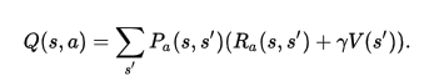
\includegraphics{img/rl1.png}
    \caption{Função que descreve o Q-Learning}
    \label{fig:figura}
\end{figure}


Enquanto que esta função é desconhecida, a experiência durante a aprendizagem é baseada nos pares (s,a)  (juntamente com os resultados de s'; isto é, "estava no estado s, executei a e s' aconteceu"). Assim, cria-se um array \textbf{Q} e usa-se as experiências para o atualizar diretamente. Isto é conhecido como \textbf{Q-Learning}.


O problema da otimização dos MDP consiste em capturar os aspetos mais importantes do problema a resolver no ambiente em que está inserido para atingir um objetivo.
O agente necessita de sentir o estado do ambiente, até um certo grau, e deve tomar ações que afetam esse estado. O agente deve ter também um ou vários objetivos, relativamente ao estado do ambiente. A formulação dos MDP pretende incluir apenas estes três aspectos: estado, ação, recompensa. Qualquer método que seja capaz de resolver este tipo de problemas, é considerado um método de aprendizagem por reforço.


\begin{figure}[H]
    \centering
    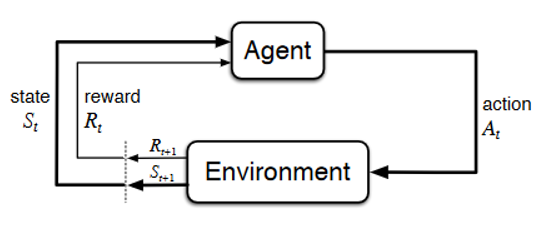
\includegraphics{img/rl2.png}
    \caption{A interação sobre ambiente de agentes na aprendizagem por reforço}
    \label{fig:figura}
\end{figure}

 A aprendizagem por reforço é diferente da aprendizagem supervisionada, uma vez que esta assenta, sobretudo na aprendizagem através de um conjunto de exemplos de treino, especificados, fornecidos por um supervisor externo. Cada exemplo contém uma descrição, e uma especificação do comportamento correto a ter para uma determinada situação. O objetivo é generalizar as respostas, de forma a agir corretamente a situações que não estão no conjunto de treino. Este é um tipo de aprendizagem importante, mas não o mais adequado para aprendizagem a partir da interação. Em território desconhecido, onde a aprendizagem se provaria mais benéfica, um agente tem de ser capaz de aprender das suas próprias experiências.

A aprendizagem por reforço é também diferente da chamada aprendizagem não supervisionada. Uma vez que, esta foca-se mais em encontrar padrões em dados não categorizados. Embora haja a tentação de considerar a aprendizagem por reforço, como aprendizagem não supervisionada, não o podemos fazer, porque não se rege por exemplos de comportamento correto. Está apenas a tentar maximizar a recompensa, e não a tentar encontrar padrões escondidos.
Por isso, é possível considerar a aprendizagem por reforço como um paradigma de "machine learning", a par da aprendizagem supervisionada e da aprendizagem não supervisionada, entre outros.

Um dos desafios que surge na aprendizagem por reforço, e não em outros tipos de aprendizagem, é o "trade-off" entre "exploration" e "exploitation". Para maximizar a recompensa, um agente deve preferir ações que já experienciou no passado e que provaram  ser eficazes em produzir uma recompensa positiva. Mas para descobrir tais ações, ele tem que tentar ações que não selecionou antes. O agente tem que explorar o que já sabe para obter a recompensa ("exploitation"), mas também tem que explorar, de forma a escolher melhor ações no futuro. O dilema é que nem a "exploration" nem a "exploitation" podem ser realizadas exclusivamente sem falhar na tarefa. O agente deve tentar uma variedade de ações e favorecer progressivamente aquelas que parecem ser melhores. Numa tarefa estocástica, cada ação deve ser testada muitas vezes para obter uma estimativa confiável da sua recompensa esperada.

\subsection{Elementos da aprendizagem por reforço:}

Para além do agente e do ambiente, é possível identificar 4 sub-elementos de um sistema de aprendizagem por reforço: a política, a recompensa, a função de valores e, opcionalmente, o modelo do ambiente.

A política define o comportamento do agente, num determinado momento. De grosso modo, é o mapeamento entre os estados percecionados do ambiente e as ações a tomar nesses estados. Em alguns casos pode ser uma simples função ou uma tabela de consulta, enquanto que noutros casos pode envolver computação extensiva, tal como um processo de procura. A política é o núcleo do agente, no sentido que, sozinha é suficiente para determinar o seu comportamento.

A recompensa define o objetivo de um problema de aprendizagem por reforço. A cada passo, o ambiente envia ao agente um valor - a recompensa. O objetivo do agente é maximizar este valor a longo prazo. Dependendo do valor da recompensa, as ações do agente são consideradas como boas ou más, e tem um papel fulcral na alteração da política.

A função de valores, ao contrário da recompensa que é imediata, específica o que é bom a longo prazo. Aproximadamente, o valor do um estado é a quantidade total de recompensa que um agente pode esperar acumular ao longo do futuro, a partir desse estado. As recompensas são, de certo modo, primárias, enquanto que os valores, como previsões de recompensas, são secundários. Sem recompensas, não poderia haver valores, e o único propósito de estimar os valore,  é para obter maiores recompensas. No entanto, é com os  valores com os quais estamos mais  preocupados ao fazer e avaliar decisões. As escolhas das ações são feitas com base em juízos de valor. Procuramos ações que geram estados de maior valor, e não a recompensa mais alta, porque essas ações obtêm a maior  recompensa a longo prazo. Infelizmente, é muito mais difícil determinar valores do que é determinar recompensas. De facto, o componente mais importante de quase todos os algoritmos de aprendizagem por reforço que consideramos é um método para estimar eficientemente os valores.

O quarto e último elemento de alguns sistemas de aprendizagem por reforço é o modelo do ambiente. Isto é algo que imita o comportamento do ambiente, e tenta prever, por exemplo, dado um estado  e uma ação, o próximo estado e a recompensa. Os métodos que usam modelos e \textbf{planeamento} são chamados métodos "model-based", em oposição aos métodos "model-free" (mais simples) que basicamente aprendem por \textbf{"tentativa e erro"}.





\subsection{Aprendizagem por reforço, um contexto real:}
 
“A aprendizagem por reforço copia um princípio muito simples da natureza, a associação de certos comportamentos com o objetivo desejado – ação e consequência.

Alguns dos primeiros investigadores na área da inteligência artificial acreditavam que este princípio poderia ser reproduzido em máquinas. Em 1951, Marvin Minsky, um estudante em Harvard, que acabaria por se tornar um dos pais da AI como professor do MIT, construiu uma máquina que usava uma forma simples de aprendizagem por reforço para imitar um rato a aprender a percorrer um labirinto. “Minsky’s Stochastic Neural Analogy Reinforcement Computer”, ou SNARC, consistia em dezenas de tubos, motores e “garras” que simulavam o comportamento de 40 neurónios e sinapses. Assim que um rato simulado escapasse do labirinto virtual, a força de algumas conexões sinápticas aumentaria, reforçando o comportamento inerente.

Houve apenas alguns sucessos nas décadas seguintes. Em 1992, Geral Tesauro, um investigador da IBM, demonstrou um programa que usava esta técnica para jogar “Gamão”. O programa ficou bom o suficiente, que podia competir com os melhores jogadores (humanos), um marco histórico para a AI. Mas a aprendizagem por reforço provou-se difícil de escalar para problemas mais complexos. “As pessoas consideravam-na uma ideia porreira, mas que não resultava mesmo”, diz David Silver, um investigador da DeepMind no Reino Unido e um dos grandes empreendedores da aprendizagem por reforço atualmente.

Mas esse ponto de vista mudou drasticamente em Março de 2016. Foi quando o AlphaGo, um programa treinado usando aprendizagem por reforço, “destruiu” um dos melhores jogadores de Go de todos os tempos, o sul coreano Lee Sedol. O acontecimento foi tão extraordinário, porque é virtualmente impossível de construir um bom programa capaz de jogar Go, usando métodos de programação convencionais. O jogo não é apenas extremamente complexo, como até grandes jogadores Go podem ter dificuldades em caracterizar certas jogadas como boas ou más, então os princípios do jogo são muito difíceis de traduzir em código. Muitos dos investigadores na área da AI estimavam que demoraria uma década para um computador jogar o jogo tão bem como um humano muito experiente.” Will Knight
